\documentclass[12pt, titlepage, a4paper]{amsart}
\usepackage[utf8]{inputenc} 
%\usepackage[magyar]{babel}
\usepackage{lmodern}
\usepackage[T1]{fontenc}
\usepackage{xcolor}

\linespread{1.43}

\usepackage{amssymb,amsmath,latexsym,amscd,url, hyperref,tikz, tikz-qtree, mathtools, cancel, amsthm, float, algpseudocode, ulem, pgf, pgfplots}
\usepackage[mathscr]{eucal}
\usepackage{pdfpages}

\theoremstyle{definition}
\newtheorem{proposition}{Proposition}
\newtheorem{conjecture}{Conjecture}
\newtheorem{descr}{Description}
\newtheorem{definition}{Definition}
\newtheorem{criterion}{Proposal}
\newtheorem{theorem}{Theorem}
\theoremstyle{theorem}
\newtheorem{lemma}{Lemma}


\theoremstyle{remark}
\newtheorem{example}{Example}

\tolerance = 9999

\textwidth = 470pt
\textheight = 650pt

\hoffset = -1.7cm
\voffset = -1.7cm

\begin{document}
\begin{definition}
Let $\Gamma\in \mathrm{Cont}$, $M\in\mathrm{Exp}$, $A\in\mathrm{Type}$, $\Gamma\vdash M:A$ is defined by recursivelly on the height of $M$:
$$\dfrac{}{\Gamma\cup\{x:A\}\vdash x:A}$$
$$\dfrac{\Gamma \vdash P:A\to B \qquad \Gamma \vdash Q:A}{\Gamma \vdash PQ:B},\qquad \dfrac{\Gamma\cup\{x:A\}\vdash P:B}{\Gamma \vdash\lambda x.P:A\to B}$$
\end{definition}
%\begin{proposition}
%Relation $\Gamma\overset{?}{\vdash} M:A$ is semi-decidable.  
%\end{proposition}
%\begin{proof}
%The following non-deterministic algorithm 
%\end{proof}
\begin{proposition}
There is an alternating polynomial time algorithm, and thus also a deterministic polynomial space algorithm to determine whether a given type $A$
is inhabited in a given basis $\Gamma$ in simply-typed lambda calculus.
\end{proposition}
\textit{Proof.} According to the Normal Form Theorem of lambda calculus, it is enough to produce a term of the long normal form:
$$\lambda x_1\dots \lambda x_n .yM_1\dots M_m$$ 
where $y$ is a variable and $M_1\dots M_m$ are in normal forms, Urzyczyn (1995).\\\\ (Without this, we only claim that among the long normal forms there the inhabitation is decidable in APTIME.)\\\\
The following procedure returns $\mathrm{inhab}_o(\Gamma\vdash ?:A)$ such that $\Gamma\vdash \mathrm{inhab}_o(\Gamma\vdash ?:A):A$ as an output, if it holds, and produces an answer “reject” otherwise.\\

\textbf{Procedure } $\mathrm{inhab}(\Gamma\vdash ?:A)$
\begin{algorithmic}
    \If{ $A$ atomic }
        \State \textbf{choose non-deterministically} $y:\; (y:A_1\to\dots\to A_m\to A)\in \Gamma$    	
    	\If{ $\exists y:\; (y:A_1\to\dots\to A_m\to A)\in \Gamma$ } 
    	
    		\If{ $\forall i=1\dots m:\;\mathrm{inhab}(\Gamma\vdash ?:A_i)$ is (\textbf{parallel}) \textbf{accepted}}
    		\State $\mathrm{inhab}(\Gamma\vdash ?:A)$ is  \textbf{accepted}
    		\State \textbf{ let} $\mathrm{inhab}_o(\Gamma\vdash ?:A)=y\,\mathrm{inhab}_o(\Gamma\vdash ?:A_1)\dots \mathrm{inhab}_o(\Gamma\vdash ?:A_m)$ 
    		\Else \quad$\mathrm{inhab}(\Gamma\vdash ?:A)$ is \textbf{ rejected}
    		\EndIf
    	\Else \quad$\mathrm{inhab}(\Gamma\vdash ?:A)$ is \textbf{ rejected}
    	\EndIf
    \ElsIf{ $A=A_1\to A_2$ }
		\State \textbf{choose non-deterministically} $x:\;(x:A_1)\in \Gamma$        
        \If{ $\exists x:\;(x:A_1)\in \Gamma$ } 	
        	\State \textbf{let} $\Gamma'=\Gamma$
        	\Else \textbf{ let} $\Gamma'=\Gamma\cup\{x:A_1\}$ with fresh $x$
    	\EndIf
    	\If{ $\mathrm{inhab}(\Gamma'\vdash ?:A_2)$ is \textbf{ accepted} }
    	\State $\mathrm{inhab}(\Gamma\vdash ?:A)$ is \textbf{accepted}
    	\State \textbf{ let }$\mathrm{inhab}_o(\Gamma\vdash ?:A)=\lambda x.\mathrm{inhab}_o(\Gamma'\vdash ?:A_2)$
    	\ElsIf{ $\mathrm{inhab}(\Gamma'\vdash ?:A_2)$ is \textbf{ rejected } }
    	\State $\mathrm{inhab}(\Gamma\vdash ?:A)$ is \textbf{ rejected }
    	\EndIf
    \EndIf
\end{algorithmic}
Informally,\\
(1) If $A$ is a type variable, or in other words an atomic type (the one that does not contain an arrow), then $M$ is an application of a variable to a sequence of terms (basically functional application defined above). We then non-deterministically choose a variable, declared in $\Gamma$ to be of type $A_1\rightarrow \dots\rightarrow A_m \rightarrow A$. If there is no such variable, we reject. If $m > 0$, we answer in parallel the questions if $A_i$ are inhabited in $\Gamma$.\\
(2) If a certain type is in the form: $A_1 \rightarrow A_2$ then the lambda expression must be an abstraction $M \equiv\lambda x.M'$, therefore we search for an $M'$ that satysfies $\Gamma, x:A_1 \vdash M':A_2$. It means that in such cases what we are supposed to do is incorporate a variable with type $A_1$ into our base and given we do that a new lambda expression $M'$ with type $A_2$ becomes derivable. The key is that upon finding out the characteristics of a certain type, the algorithm decides whether the preconditions and the route for that type are satysfied. The reason why it is a polynomial time procedure is that the number of steps the algorithm takes only grows by at most a quadratic rate as a function of context size.\\\\
The size of the input is the number of sub-formulas in $\Gamma\cup\{A\}$, say $n$. We have to give an upper bound for the length of the longest computational path. Suppose, $\alpha$ is a universal state in the case ``$A$ is atomic'' and the question is whether $\mathrm{inhab}(\Gamma'\vdash ?:A_i')$ is accepted for all $i=1...m$ or not. If $\beta$ is also an ``$A$ is atomic'' case ($\beta_1$) or an existential state in the compound ``$A=A_1\to A_2$'' case ($\beta_2$), then $\Gamma$ remains unchanged and the number of such transitions (with unchanged $\Gamma'$) is not greater than the number of questions of the form $\Gamma'\vdash ?:B$ where $\Gamma'$ is fixed, i.e. the number of all subformulas in the original $\Gamma\cup \{A\}$ which is $n$. If $\gamma$ is a state in the compound ``$A=A_1\to A_2$'' case and $\Gamma''=\Gamma'\cup\{x:A_2\}$ is a proper expansion, then \textit{along one computational path,} the number of such expansions is not greater than the number of all subformulas in the original $\Gamma\cup \{A\}$, i.e. $n$. Hence, the depth of recursion is at most the number of possible proper expansions times the number of questions in a given expansion, i.e. $n^2$.
\begin{center}
\resizebox{0.5\textwidth}{!}{
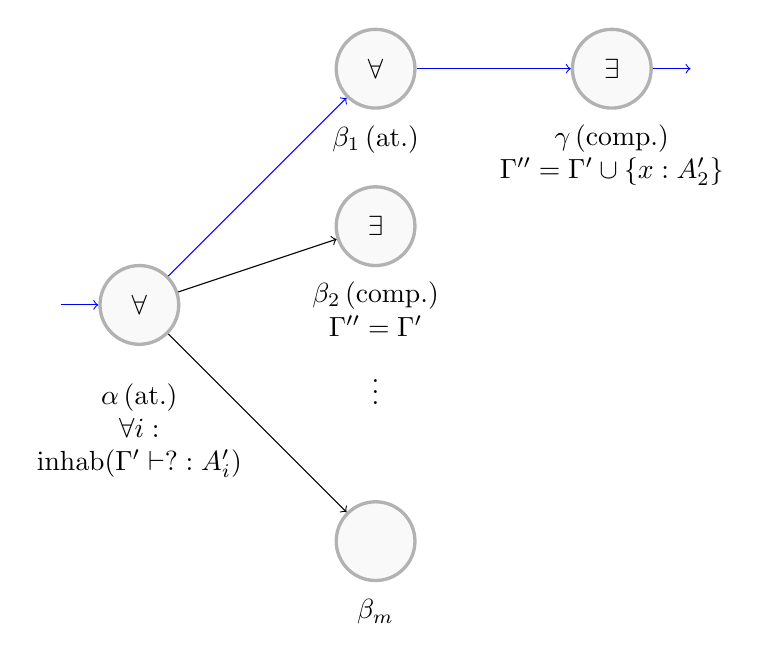
\begin{tikzpicture}[
roundnode/.style={circle, draw=gray!60, fill=gray!5, very thick, minimum size=10mm}
]
%Nods
\draw (1,0) node [roundnode]        (centralcircle)       {$\forall$};
\draw (1,-1.6) node  {$\begin{matrix}\alpha\,\mbox{(at.)}\\\forall i:\\\mathrm{inhab}(\Gamma'\vdash ?:A_i')\end{matrix}$};

\draw (4,3) node[roundnode]        (r1)  {$\forall$};
\draw (4,2.1) node  {$\beta_1\,\mbox{(at.)}$};

\draw (4,1) node[roundnode]        (r2)  {$\exists$};
\draw (4,-0.1) node  {$\begin{matrix}\beta_2\,\mbox{(comp.)}\\\Gamma''=\Gamma'\end{matrix}$};

\draw (4,-1) node       (r3) {$\vdots$};

\draw (4,-3) node[roundnode]        (r4) {};
\draw (4,-3.9) node  {$\beta_m$};

\draw (7,3) node[roundnode]       (rr1)  {$\exists$};
\draw (7,1.9) node  {$\begin{matrix}\gamma\,\mbox{(comp.)}\\\Gamma''=\Gamma'\cup\{x:A_2'\}\end{matrix}$};


%Lines
\draw[->, color=blue] (0,0) -- (centralcircle);
\draw[->, color=blue] (centralcircle) -- (r1);
\draw[->] (centralcircle) -- (r2);
\draw[->] (centralcircle) -- (r4);
\draw[->, color=blue] (r1) -- (rr1);
\draw[->, color=blue] (rr1) -- (8,3);
\end{tikzpicture}}
\end{center}
$\square$\\

The above PTIME \textit{alternating} algorithm employs two magicians. One works in case (1), who gives us the lucky path leading us to the answer “accept”, and the other one in case (2), leading us to the answer “reject”. This is crucial because otherwise the number of steps during the solution is much larger, hence the distinction in the proposition, “alternating polynomial time and deterministic polynomial space” algorithms.
\begin{proposition} There is an alternating linear time algorithm deciding whether the relation 
$$\Gamma\vdash N:A$$ 
holds or not, if context $\Gamma$, \textit{normal} expression $N$, and type $A$ are given.   
\end{proposition}
\begin{proof} Realization of type checking of a normal expression:
\begin{itemize}
\item[] \textit{Input:} $\Gamma, N, A$, where $N$ is normal.
\begin{itemize}
\item[] \textit{Input size:} the height $|N|$ of the syntax tree of $N$.
\end{itemize}
\item[] \textit{Output:} the Boolean value \textbf{accept}$\slash$\textbf{reject}. 
\end{itemize}
Procedure $\mathsf{typecheck}_a$ accepts the input $(\Gamma,N,A)$ iff $\Gamma\vdash N:A$ holds. 

\par \textbf{procedure} $\mathsf{typecheck}_a$
\begin{center}
\boxed{
\resizebox{.6\textwidth}{!}{
\begin{minipage}{.8\textwidth}

\begin{algorithmic}
    \If{ $N=\lambda x.N'$} 
    	\If{ $A=A_1\to A_2$} 
    		\State \textbf{do} $\mathsf{typecheck}_a(\Gamma\cup \{x:A_1\}, N', A_2)$
    			\If{ $\mathsf{typecheck}_a\mbox{ \textbf{accepts} }(\Gamma\cup \{x:A_1\}, N', A_2)$ } 
    			\State \textbf{ accept } $(\Gamma,N,A)$
    				\Else \textbf{ reject } $(\Gamma,N,A)$  
    			\EndIf  		
    	\Else \textbf{ reject } $(\Gamma,N,A)$
    	\EndIf
    \ElsIf{ $N=N'N''$ }
    \State \textbf{choose non-deterministically} $A_3\in \mathrm{Sub}(\Gamma\cup \{A\})$ such that\\
        \qquad\qquad$\begin{cases}\mathsf{typecheck}_a\mbox{ \textbf{accepts} } (\Gamma, N',A_3\to A)\;\mbox{ and }\\
        \mathsf{typecheck}_a\mbox{ \textbf{accepts} } (\Gamma, N'',A_3) \end{cases}$
        \If{ it is \textbf{successful} } \textbf{ accept }$(\Gamma,N,A)$
        \Else  \textbf{ reject }$(\Gamma,N,A)$
        \EndIf
    \ElsIf{ $N=x$ }
    \State\textbf{choose non-deterministically} $x$ such that  $(x:A)\in \Gamma$ 
    \If { it is \textbf{successful} } \textbf{ accept} $(\Gamma, N,A)$
    \Else \;\textbf{ reject} $(\Gamma, N,A)$
	\EndIf
\EndIf
\end{algorithmic}

\end{minipage}
}}

\end{center}The depth of recursion is preciselly $|N|$, hence the alternating algorithm's runtime is  $\boxed{\mathcal{O}(|N|)}$
\end{proof}
\begin{conjecture}  There is a deterministic fixed parameter linear algorithm deciding whether the relation 
$$\Gamma\vdash N:A$$ 
holds or not, if context $\Gamma$, \textit{normal} expression $N$, and type $A$ are given.
\end{conjecture}$ $\\
\noindent Realization of type checking of a normal expression:
\begin{itemize}
\item[] \textit{Input:} $\Gamma, N, A$, where $N$ is normal.
\begin{itemize}
\item[] \textit{Parameter:} $k=|\mathrm{Sub}(\Gamma\cup \{A\})|$\quad (the number of subformulas in $\Gamma\cup \{A\}$)
\item[] \textit{Input size:} the height $|N|$ of the syntax tree of $N$.
\end{itemize}
\item[] \textit{Output:} the Boolean value \textbf{accept}$\slash$\textbf{reject}. 
\end{itemize}
Procedure $\mathsf{typecheck}_p$ accepts the input $(\Gamma,N,A)$ iff $\Gamma\vdash N:A$ holds.\\\\
The runtime of $\mathsf{typecheck}_p$ is less than $\boxed{2k^2\cdot |N|}$.\\\\
\begin{conjecture} There is a PTIME algorithm deciding whether the relation 
$$\Gamma\vdash N:A$$ 
holds or not, if context $\Gamma$, \textit{normal} expression $N$, and type $A$ are given.
\end{conjecture}$ $\\
\noindent Realization of type checking of a normal expression:
\begin{itemize}
\item[] \textit{Input:} $\Gamma, N, A$, where $N$ is normal.
\begin{itemize} 
\item[] \textit{Input size:} $n=\max\{|\mathrm{Sub}(\Gamma\cup \{A\})|,|N|\}$
\end{itemize}
\item[] \textit{Output:} the Boolean value \textbf{accept}$\slash$\textbf{reject}. 
\end{itemize}
Procedure $\mathsf{typecheck}_d$ accepts the input $(\Gamma,N,A)$ iff $\Gamma\vdash N:A$ holds.\\\\
The runtime of $\mathsf{typecheck}_d$ is less than $\boxed{2|N|^3}$.



\end{document}





















\begin{proposition}
There is an alternating polynomial time algorithm, and thus also a deterministic polynomial space algorithm to determine whether a given type $A$
is inhabited in a given basis $\Gamma$ in simply-typed lambda calculus.
\end{proposition}
\textit{Proof.} According to the Normal Form Theorem of lambda calculus, it is enough to produce a term of the form:
$$\lambda x_1\dots \lambda x_n .yM_1\dots M_m$$ 
where $y$ is a variable and $M_1\dots M_m$ are in normal forms, Urzyczyn (1995). The following procedure returns $\mathrm{inhab}_o(\Gamma\vdash ?:A)$ such that $\Gamma\vdash \mathrm{inhab}_o(\Gamma\vdash ?:A):A$ as an output, if it holds, and produces an answer “reject” otherwise.\\

\textbf{Procedure } $\mathrm{inhab}(\Gamma\vdash ?:A)$
\begin{algorithmic}
    \If{ $A$ atomic }
    	\If{ $\exists y:\; (y:A_1\to\dots\to A_m\to A)\in \Gamma$ } 
    	\State \textbf{choose non-deterministically} $y:\; (y:A_1\to\dots\to A_m\to A)\in \Gamma$
    	\For{ $i=1\dots m$ } $\mathrm{inhab}(\Gamma\vdash ?:A_i)$
    	\EndFor
    	\If{ $\forall i=1\dots m:\;\mathrm{inhab}(\Gamma\vdash ?:A_i)$ is \textbf{accepted}}
    	\State $\mathrm{inhab}(\Gamma\vdash ?:A)$ is \textbf{accepted}
    	\State \textbf{ let} $\mathrm{inhab}_o(\Gamma\vdash ?:A)=y\,\mathrm{inhab}_o(\Gamma\vdash ?:A_1)\dots \mathrm{inhab}_o(\Gamma\vdash ?:A_m)$ 
    	\Else \quad$\mathrm{inhab}(\Gamma\vdash ?:A)$ is \textbf{ rejected}
    	\EndIf
    	\Else \quad$\mathrm{inhab}(\Gamma\vdash ?:A)$ is \textbf{ rejected}
    	\EndIf
    \ElsIf{ $A=A_1\to A_2$ }
        \If{ $\exists x:\;(x:A_1)\in \Gamma$ } 
        \State \textbf{choose non-deterministically} $x:\;(x:A_1)\in \Gamma$
        \State \textbf{let} $\Gamma'=\Gamma$
        \Else \textbf{ let} $\Gamma'=\Gamma\cup\{x:A_1\}$ with fresh $x$
    	\EndIf
    	\State \textbf{do} $\mathrm{inhab}(\Gamma'\vdash ?:A_2)$
    	\If{ $\mathrm{inhab}(\Gamma'\vdash ?:A_2)$ is \textbf{ accepted} }
    	\State $\mathrm{inhab}(\Gamma\vdash ?:A)$ is \textbf{accepted}
    	\State \textbf{ let }$\mathrm{inhab}_o(\Gamma\vdash ?:A)=\lambda x.\mathrm{inhab}_o(\Gamma'\vdash ?:A_2)$
    	\ElsIf{ $\mathrm{inhab}(\Gamma'\vdash ?:A_2)$ is \textbf{ rejected } }
    	\State $\mathrm{inhab}(\Gamma\vdash ?:A)$ is \textbf{ rejected }
    	\EndIf
    \EndIf
\end{algorithmic}
The size of the input is the number of sub-formulas in $\Gamma\cup\{A\}$, say $n$. It is easy to see that the number of recursive calls “$\mathrm{inhab} (\Delta\vdash ?:B)$” during the algoritm, is less than $n^2$. If we look at the algorithm in what form it puts question $\Delta\vdash ?:B$, we can see the following. $B$ is always belongs to the set of sub-formulas of $\Gamma\cup\{A\}$. $\Delta$ is a finite extension of $\Gamma$, with at most one formula per recursion, form the set of sub-formulas of $\Gamma\cup\{A\}$. Hence, there are at most $n\cdot n=n^2$ \textit{distinct} questions of the form $\Delta\vdash ?:B$ during the algorithm, which can be decided by at most $n^2$ calls of procedure $\mathrm{inhab}$. This means that, the runtime of this procedure is $O(n^2)$. Since $\mathrm{APTIME}\subseteq\mathrm{PSPACE}$, the decision problem above is a polynomial space problem.\\
Informally,\\
(1) If $A$ is a type variable, or in other words an atomic type (the one that does not contain an arrow), then $M$ is an application of a variable to a sequence of terms (basically functional application defined above). We then non-deterministically choose a variable, declared in $\Gamma$ to be of type $A_1\rightarrow \dots\rightarrow A_m \rightarrow A$. If there is no such variable, we reject. If $m > 0$, we answer in parallel the questions if $A_i$ are inhabited in $\Gamma$.\\
(2) If a certain type is in the form: $A_1 \rightarrow A_2$ then the lambda expression must be an abstraction $M \equiv\lambda x.M'$, therefore we search for an $M'$ that satysfies $\Gamma, x:A_1 \vdash M':A_2$. It means that in such cases what we are supposed to do is incorporate a variable with type $A_1$ into our base and given we do that a new lambda expression $M'$ with type $A_2$ becomes derivable. The key is that upon finding out the characteristics of a certain type, the algorithm decides whether the preconditions and the route for that type are satysfied. The reason why it is a polynomial time procedure is that the number of steps the algorithm takes only grows by at most a quadratic rate as a function of context size.$\square$\\

The above PTIME \textit{alternating} algorithm employs two magicians. One works in case (1), who gives us the lucky path leading us to the answer “accept”, and the other one in case (2), leading us to the answer “reject”. This is crucial because otherwise the number of steps during the solution is much larger, hence the distinction in the proposition, “alternating polynomial time and deterministic polynomial space” algorithms.
